\documentclass[aspectratio=1610]{beamer}
%[aspectratio=169]
% ------------------------------------------------------------------------
% PRAESENTATIONSAUSWAHL
\usecolortheme[RGB={3,138,94}]{structure} 
\mode<presentation> {
	%\usetheme{CambridgeUS} 
	\usetheme{Warsaw} 
	% oder Antibes, Bergen, Berkeley, ....
	
	%\setbeamercovered{transparent}
	
}
\useoutertheme{infolines}
\setbeamertemplate{headline}{}

\beamertemplatenavigationsymbolsempty
\definecolor{unigruen}{RGB}{3,138,94} 

\usefonttheme{professionalfonts}  % Aenderung der Schriftart
% (bei mathematischen Ausdruecken)
% ------------------------------------------------------------------------


% ------------------------------------------------------------------------
% EINGEBUNDENE PAKETE
\usepackage{xcolor}
\usepackage{varwidth}
\usepackage[utf8]{inputenc}
\usepackage{times,relsize,xspace}
\usepackage[T1]{fontenc}
\usepackage{mathtools}
\usepackage{dirtytalk}
\usepackage{minted,hyperref}

\hypersetup{
	colorlinks   = true,
}

\usepackage[style=authortitle,]{biblatex} %Imports biblatex package
\addbibresource{bibliography.bib} %Import the bibliography file
% Oder was auch immer. Zu beachten ist, das Font und Encoding passen
% muessen. Falls T1 nicht funktioniert, kann man versuchen, die Zeile
% mit fontenc zu loeschen.
% ------------------------------------------------------------------------

\newtheorem{thm}{Theorem}[theorem]

% ------------------------------------------------------------------------

\newcommand{\Rplus}{\protect\hspace{-.1em}\protect\raisebox{.35ex}{\smaller{\smaller\textbf{+}}}}
\newcommand{\Cpp}{\mbox{C\Rplus\Rplus}\xspace}

% Define the centeredblock environment to accept an optional argument for width
\newenvironment{centeredblock}[2][0.8\textwidth]
{ % This code will be executed at the beginning of the environment
	\begin{center}
		\begin{varwidth}{#1} % Use the argument for width
			\begin{block}{#2}
				\centering
			}
			{ % This code will be executed at the end of the environment
			\end{block}
		\end{varwidth}
	\end{center}
}


\title{Parallel Debugging}
\subtitle{}
\author{Jonathan Schmalfuß}
\institute[UBT]{Chair of Scientific Computing \\ University of Bayreuth}
\date{\today}
%\tiny A talk adapt from \href{hackingcpp.com}{hackingcpp}
\begin{document}
	
	% TITELSEITE
	{
		\setbeamertemplate{headline}{} % Bei der Titelseite keine Kopf- und
		\setbeamertemplate{footline}{} % Fusszeile
		\begin{frame}
			\pagestyle{empty}
			\titlepage
			\pagestyle{empty}
		\end{frame}
	}
	
	\logo{} % remove logo from all following pages
	% Titelseite bei der Nummerierung ignorieren
	\addtocounter{framenumber}{-1}
	\setminted{fontsize=\footnotesize}
	
	\begin{frame}[fragile]{Parallel debugging}
		\begin{centeredblock}{}
			\say{Sequential programming is really hard, and parallel programming is a step beyond that.} - Andrew S. Tanenbaum, professor at Vrije Universiteit Amsterdam
		\end{centeredblock}
		
		\begin{centeredblock}{}
			\say{Debugging is twice as hard as writing the code in the first place. Therefore, if you write the code as cleverly as possible, you are, by definition, not smart enough to debug it.} - Brian Kernighan, professor at Princeton University.
		\end{centeredblock}
	\end{frame}
	
	\begin{frame}[fragile]{Techniques in general}
		\begin{centeredblock}{}
			\say{Most bugs also appear in the sequential version of the code} - me 
		\end{centeredblock}
		
		\pause
		\begin{centeredblock}{Distinguish Problem}
			\begin{columns}
				\hfill
				\begin{column}{0.15 \textwidth}
					\begin{block}{}
						Sequential Problem
					\end{block}
				\end{column}
				\hfill
				$\xLeftarrow[\text{persists}]{\text{problem}}$ 
				\hfill
				\begin{column}{0.3 \textwidth}
					\begin{block}{}
						Force Sequential Execution via \texttt{MPI\_Barrier()}
					\end{block}
				\end{column}
				\hfill
				$\xRightarrow[\text{now}]{\text{works}}$
				\hfill
				\begin{column}{0.15 \textwidth}
					\begin{block}{}
						Parallel Problem
					\end{block}
				\end{column}
				\hfill
			\end{columns}
		\end{centeredblock}
		\pause
		\begin{centeredblock}[0.95 \textwidth]{The experts opinion: Anthony Williams - author/ coauthorof the thread library in \Cpp}
			\begin{enumerate}
				\item Reviewing code to locate potential bugs
				\item Locating concurrency-related bugs by testing / Designing for testability
			\end{enumerate}
		\end{centeredblock}
	\end{frame}
	
	\begin{frame}[fragile]{Questions while reviewing multiprocess code}
		\begin{centeredblock}{}
			\begin{itemize}
				\item Are there any ordering requirements between the operations done in this
				process and those done in another? How are those requirements enforced?
				\item Which data needs to be protected from concurrent access? How do you ensure that the data is protected?
				\item Where in the code could other processes be at this time?
				\item Is the data loaded by this process still valid? 
				\item If you assume that another process could be modifying the data, what would that
				mean and how could you ensure that this never happens?
			\end{itemize}
		\end{centeredblock}
	\end{frame}
	
	\begin{frame}[fragile]{Parallel Debugging: How to?}
			\begin{columns}
				\hfill
				\begin{column}{0.3\textwidth}
					\begin{centeredblock}{the easy way}
						\begin{itemize}
							\item use a debugger and or fronted made for debugging MPI code
							\item Industry Standard: \href{https://www.linaroforge.com/}{ddt}\footnotemark, \href{https://totalview.io/}{TotalView}\footnotemark[1]
						\end{itemize}
					\end{centeredblock}
				\end{column}
				\hfill
				\begin{column}{0.7\textwidth}
					\begin{centeredblock}{should-always-work way}
						\begin{itemize}
							\item mininmal requirements: a debugger (gdb) + a way of finding the running processes (ps/top)
							\item \texttt{mpirun} creates multiple processes --> attach to relevant processes or all --> debugg each of them sequentially
							\item limits: low number of processes, requires duplicating input for each process
						\end{itemize}
					\end{centeredblock}
				\end{column}
				\hfill
			\end{columns}
		
		\begin{centeredblock}{Compromise? Open Source Projects / Free:}
			command line tool with plotting ability \href{https://github.com/TomMelt/mdb?tab=readme-ov-file}{mdb}, intel oneAPI with \href{https://www.intel.com/content/www/us/en/docs/distribution-for-gdb/tutorial-debugging-dpcpp-linux/2024-1/debugging-mpi-programs.html}{mpigdb} or a shell script \href{https://github.com/Azrael3000/tmpi}{tmpi}
		\end{centeredblock}

		
			\footnotetext{temporary free / student license available }
	\end{frame}
	
	\begin{frame}[fragile]{MPI debugging - should-always-work}
		\begin{centeredblock}{Debug Deadlocks: Attach to the process [Live-session]}
			Situation: you have a deadlock, i.e. your executable is stuck
			\begin{enumerate}
				\item Compile with debug flags: \texttt{mpic++ -g -Wall <file> -o <name>}
				\item Wait until stuck
				\item Figure out process id's via \texttt{top} or \texttt{ps -a | grep <name>}
				\item Attach to the process and see where you are stuck --> figure out what the problem is
			\end{enumerate}
		\end{centeredblock}
	\end{frame}

	\begin{frame}[fragile]{Recap Live-Session: MPI debugging - should-always-work}
		\begin{centeredblock}{}
			\begin{minted}[autogobble, breaklines]{sh}
				$ mpic++ deadlock_blocking_recieve_before_send.cpp -g -Wall
				$ mpirun -np 2 ./a.out 10
				0: Receiving 10 elements of type int from my left neighbor 1.
				1: Receiving 10 elements of type int from my left neighbor 0.
			\end{minted}
		\end{centeredblock}
		
		\begin{centeredblock}{}
			\begin{minted}[autogobble]{sh}
				$ ps -a | grep a.out
				553640 pts/1    00:00:15 a.out
				$ ps -a | grep a.out
				553980 pts/1    00:00:02 a.out
				553981 pts/1    00:00:02 a.out
				$ gdb -p 553980
				GNU gdb (Ubuntu 12.1-0ubuntu1~22.04.2) 12.1
				...
				(gdb) where
				#0  in opal_progress () from ...
				#1  in mca_pml_ob1_recv () from ...
				#2  in PMPI_Recv () from ...
				#3  in main () at deadlock_blocking_recieve_before_send.cpp:28
			\end{minted}
		\end{centeredblock}
	\end{frame}

	\begin{frame}[fragile]{MPI debugging - multiple instances}
		\begin{centeredblock}{Attaching debugger to serval instances of the executable [Live-session]}
			\begin{itemize}
				\item Use mpirun to launch separate instances of serial debuggers
				\item Drawback: many process, usually problematic
			\end{itemize}
			\href{https://www.open-mpi.org/faq/?category=debugging#serial-debuggers}{OpenMPI: FAQ: Debugging applications in parallel}
			
			\begin{itemize}
				\item Attach a terminal with gdb to each process (opens multiple windows using xterm)
				\mintinline{sh}{mpiexec -n 2 xterm -e gdb --args a.out 10}
				\item Attach to single process from the beginning with arguments: \mintinline{sh}{mpirun -n 1 gdb --args ./a.out 10 : -n 1 ./a.out 10}
				\item Attach to single process with xterm from the beginning with arguments: \mintinline{sh}{mpirun -n 1 xterm -e gdb --args ./a.out 10 : -n 1 ./a.out 10}
			\end{itemize}
		\end{centeredblock}
	\end{frame}

	\begin{frame}[fragile]{Recap Live-Session: MPI debugging - multiple instances}
		\begin{centeredblock}{}
			\begin{minted}[autogobble, breaklines]{sh}
				$ mpicxx -g simple-mpi.cpp
				$ mpirun -n 2 xterm -e gdb --args a.out 10
			\end{minted}
			\vspace{-0.5cm}
			\begin{columns}
				\begin{column}{0.5 \textwidth}
					\centering
					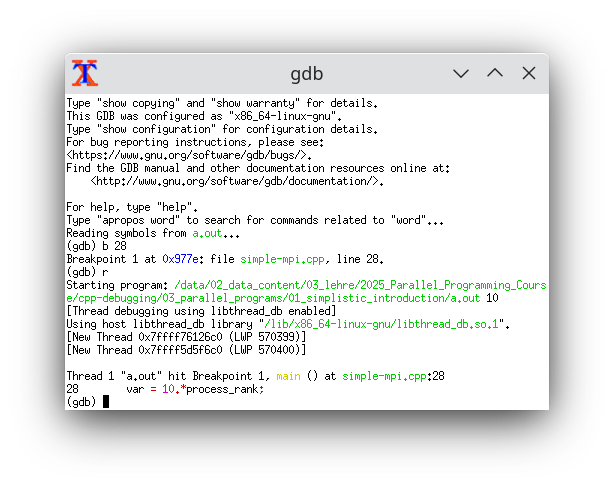
\includegraphics[width=0.7\linewidth]{figures/gdb-xterm-window-0}
				\end{column}
				\begin{column}{0.5 \textwidth}
					\centering					
					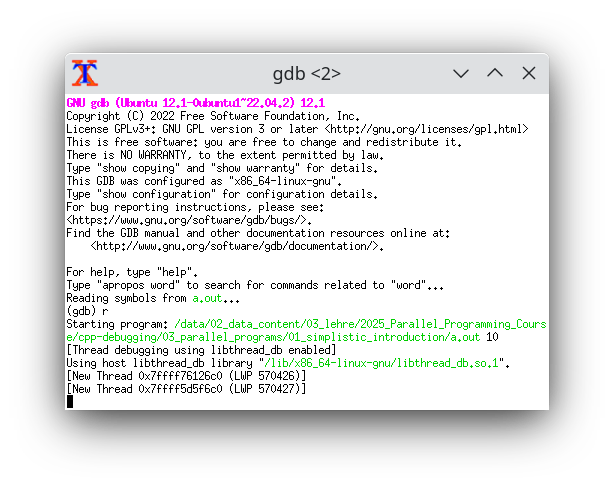
\includegraphics[width=0.7\linewidth]{figures/gdb-xterm-window-1}
				\end{column}
			\end{columns}
			\vspace{-0.5cm}
		\end{centeredblock}
		
		\begin{centeredblock}{}
			\begin{minted}[autogobble]{sh}
				$ mpicxx -g simple-mpi.cpp
				$ mpirun -n 1 gdb --args ./a.out 10 : -N 1 ./a.out 10
				GNU gdb
				(gdb) b 28
				Starting program: /data/01_simplistic_introduction/a.out 10
				[New Thread 0x7ffff76126c0 (LWP 572127)]
				[New Thread 0x7ffff5d5f6c0 (LWP 572128)]
				
				Thread 1 "a.out" hit Breakpoint 1, main () at simple-mpi.cpp:28
				28        var = 10.*process_rank;
			\end{minted}
		\end{centeredblock}
	\end{frame}

	\begin{frame}[fragile]{MPI debugging - mgdb}
		\begin{centeredblock}{mgdb [Live-session]}
			\begin{itemize}
				\item easy installable : \begin{minted}{sh}
python3 -m venv .mdb
source .mdb/bin/activate
pip install mdb-debugger[termgraph]
				\end{minted} 
				\item potentially powerful
				\item drawback: is command line only / early development stages
				\item \href{https://mdb.readthedocs.io/en/latest/quick-start.html}{QuickStart}
			\end{itemize}
		\end{centeredblock}
	\end{frame}

\begin{frame}[fragile]{Recap Live-Session: MPI debugging - mgdb}
	\begin{centeredblock}{}
		\begin{minted}[autogobble]{sh}
			$ python3 -m venv .mdb
			$ source .mdb/bin/activate
			$ pip install mdb-debugger[termgraph]
			...
			$ mpicxx -g simple-mpi.cpp 
			$ mdb launch -b gdb -n 2 -t ./a.out --log-level=DEBUG
			running on host: 132.180.176.41
			to connect to the debugger run:
			mdb attach -h 132.180.176.41 -p 2000
			...
		\end{minted}
	\end{centeredblock}
	\begin{centeredblock}[0.95 \textwidth]{}
		\begin{minted}[autogobble]{sh}
			$ source .mdb/bin/activate
			$ mdb attach -h 132.180.176.41 -p 2000
			(mdb 0-1) command 0 b 38
			0:      Breakpoint 2: file simple-mpi.cpp, line 39.
			(mdb 0-1) broadcast start
			(bcm 0-1) c
			^C0:    Continuing.
			0:      process 0 sleeping for 3s...
			0:      Thread 1 "a.out" hit Breakpoint 2, main () at simple-mpi.cpp:39
			0:      39        MPI_Barrier(MPI_COMM_WORLD);
			************************************************************************
			1:      Continuing.
			1:      ^C
			1:      Thread 1 "a.out" received signal SIGINT, Interrupt.
			1:      0x00007ffff7e68fa0 in opal_progress@plt () from /lib/x86_64-linux-gnu/libmpi.so.40
			1:
			1:      Interrupted: True
			
			(bcm 0-1) where
			0:      #0  main () at simple-mpi.cpp:39
			************************************************************************
			1:      #0  0x00007ffff7e68fa0 in opal_progress@plt () from 
			1:      #3   in PMPI_Barrier () from /lib/x86_64-linux-gnu/libmpi.so.40
			1:      #4   in main () at simple-mpi.cpp:39
		\end{minted}
	\end{centeredblock}
\end{frame}

	\begin{frame}[fragile]{MPI debugging: Memchecker}
		\begin{centeredblock}[0.85 \textwidth]{}
			\begin{itemize}
				\item Requires: Open MPI 1.3 or later, and Valgrind 3.2.0 or later
				\item Otherwise: works, but with many false positives
				\item Needs to be enable at compilation state of OpenMPI, unfortunately often is not
				\item to enable locally, see \href{https://www.open-mpi.org/faq/?category=debugging#memchecker}{How can I use Memchecker}
				\item \begin{minted}[tabsize=2,breaklines]{sh}
mpirun -np 2 valgrind --suppressions=$PREFIX/share/openmpi/openmpi-valgrind.supp <executable name>
				\end{minted}
			\end{itemize}
		\end{centeredblock}
	\end{frame}
	
	\begin{frame}[fragile]{The easy way}
		\begin{centeredblock}{}
			\centering					
			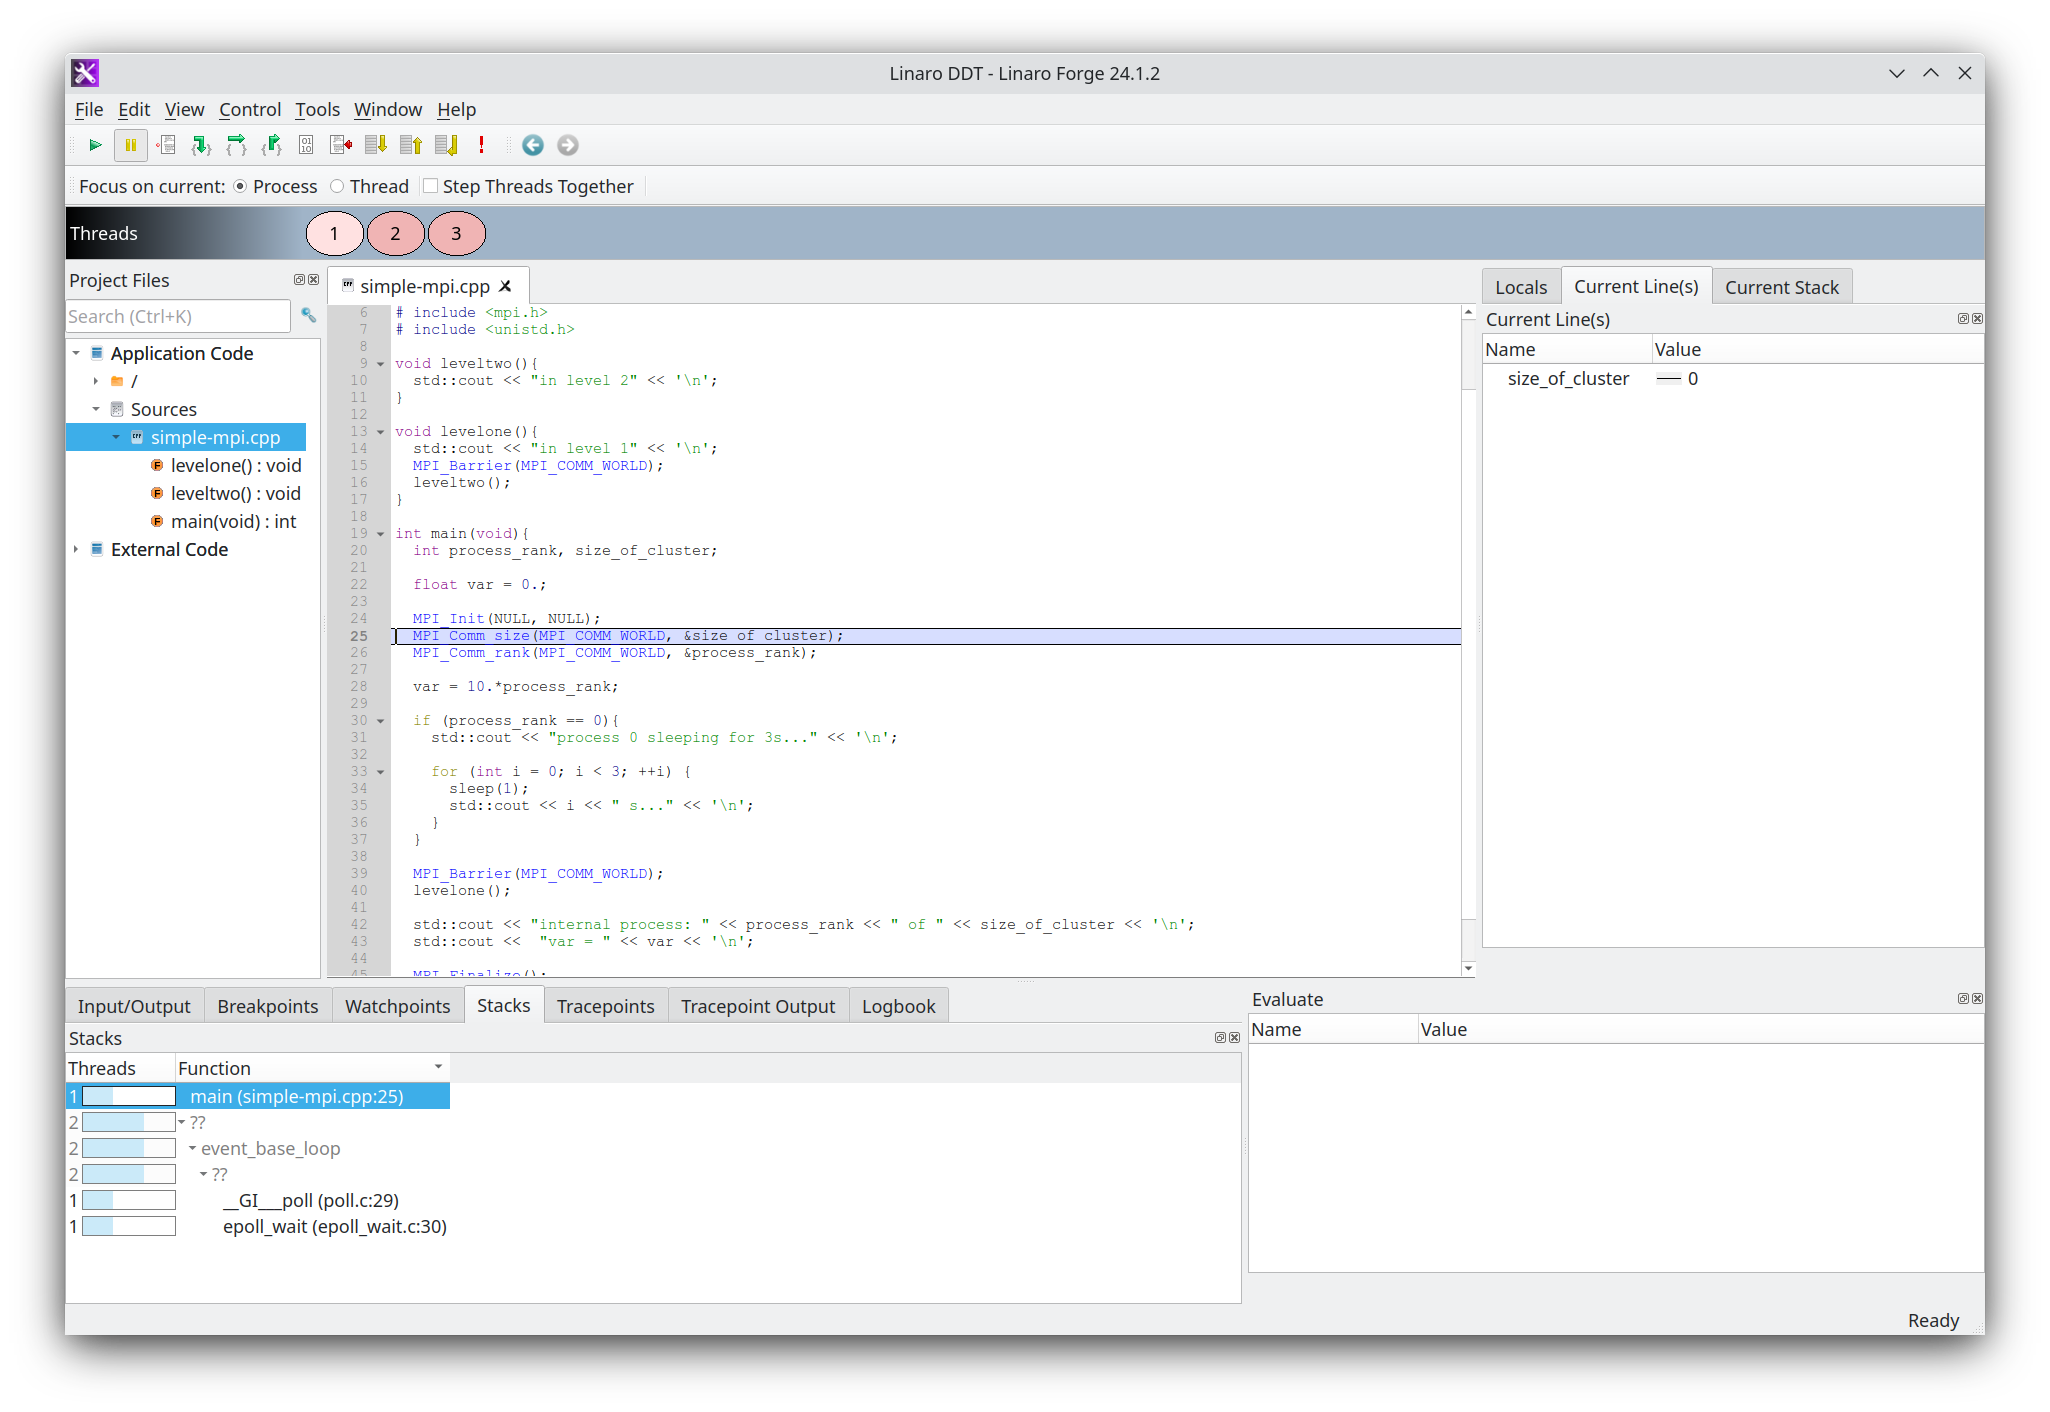
\includegraphics[width=0.9\linewidth]{figures/ddt}
			
			
			\href{https://youtu.be/Q8HwLg22BpY?t=1006}{ddt tutorial}
		\end{centeredblock}
	\end{frame}
	
	\begin{frame}[fragile]{Now what?}
		\begin{block}{Use the tools / test them on simple and more complex examples}
			In the corresponding \href{https://github.com/joscao/cpp-debugging}{github project} work through the folder \texttt{03\_parallel\_programs} content. The available tools on the PC-Pool workstations are gdb / xterm.
			
			\vspace{1cm}
			
			Possible tasks:
			\begin{itemize}
				\item Attach gdb in different ways to the same executable!
				\item Is it a sequential or parallel problem?
				\item Last but not least: Ask Questions, not only to me but also to each other about your understanding.
			\end{itemize}
		\end{block}
	\end{frame}
\end{document}